\documentclass[english,12pt,a4paper,pdftex,sci,utf8]{./styles/aaltothesis}
\usepackage{graphicx}
\usepackage{ifpdf}
\ifpdf
   % put here packages only for the PDF:
   \DeclareGraphicsExtensions{.pdf,.png,.jpg,.mps}
   \usepackage{hyperref}
\else
   % put here packages only for the DVI:
\fi

% put all the other packages here:
\usepackage{./styles/clemens_thesis}

% \includeonly{./tex/preamble, ./tex/background }

\begin{document}

% !TEX root = ../thesis.tex
% !TEX spellcheck = en-US

\university{Aalto University}
\school{School of Science}

\department{Department of Information and Computer Science}
\professorship{Machine Learning, Data Mining, and Probabilistic Modeling}

\univdegree{MSc}

\author{Clemens Westrup}

%% Your thesis title comes here and again before a possible abstract.
%% If the title is very long and latex does an
%% unsatisfactory job of breaking the lines, you will have to force a
%% linebreak with the \\ control character.
%% Do not hyphenate titles.
%%
% \thesistitle{From a fragmented process towards integrated end-to-end learning: An explorative study of the evolution of text classification approaches towards Deep Learning}
\thesistitle{Something something}

\place{Espoo}

\date{16.1.2015}

%% B.Sc. or M.Sc. thesis supervisor
%% Note the "\" after the comma. This forces the following space to be
%% a normal interword space, not the space that starts a new sentence.
%% This is done because the fullstop isn't the end of the sentence that
%% should be followed by a slightly longer space but is to be followed
%% by a regular space.
%%
\supervisor{Prof.\ Aristides Gionis}

%% B.Sc. or M.Sc. thesis advisors(s). You can give upto two advisors in
%% this template. Check with your supervisor how many official advisors
%% you can have.
%%
\advisor{Clemens Westrup}
% \advisor{Michael Mathioudakis, Ph.D.}
%\advisor{M.Sc.\ Polli Pohjaaja}

%% Aalto logo: syntax:
%% \uselogo{aaltoRed|aaltoBlue|aaltoYellow|aaltoGray|aaltoGrayScale}{?|!|''}
%%
%% Logo language is set to be the same as the document language.
\uselogo{aaltoYellow}{!}

%% Create the coverpage
%%
\makecoverpage

%% English abstract.
%% All the information required in the abstract (your name, thesis title, etc.)
%% is used as specified above.
%% Specify keywords
%%
%%
\keywords{NLP, bla bla, keyword}
%% Abstract text
\begin{abstractpage}[english]
  Your abstract in English. Try to keep the abstract short; approximately
  100 words should be enough. The abstract explains your research topic,
  the methods you have used, and the results you obtained.
  Your abstract in English. Try to keep the abstract short; approximately
  100 words should be enough. The abstract explains your research topic,
  the methods you have used, and the results you obtained.

  Your abstract in English. Try to keep the abstract short; approximately
  100 words should be enough. The abstract explains your research topic,
  the methods you have used, and the results you obtained.
  Your abstract in English. Try to keep the abstract short; approximately
  100 words should be enough. The abstract explains your research topic,
  the methods you have used, and the results you obtained.
\end{abstractpage}

%% Force a new page so that the possible English abstract starts on a new page
\newpage


%% Preface
\mysection{Preface}
% - Michael: for all the incredible support, patience, interest and caring
% - Aris: for providing me with this amazing opportunity to do this
% - Juho: for introducing me to proper scientific work
% - Henning: for discussions, a great friendship
% - Martti: for being an awesome friend
% - my family: for something something
% - Mikko
% - Mika
% - Sami and Hugo
I want to thank some people \ldots
\\

\vspace{5cm}
Helsinki, 30.08.2016

\vspace{5mm}
{\hfill Clemens Westrup \hspace{1cm}}

%% Force new page after preface
\newpage

%% Table of contents.
\thesistableofcontents


%% Symbols and abbreviations
\mysection{Symbols and abbreviations*}

% \subsection*{Symbols*}
%
% \begin{tabular}{ll}
% $\mathbf{B}$  & magnetic flux density  \\
% $c$              & speed of light in vacuum $\approx 3\times10^8$ [m/s]\\
% $\omega_{\mathrm{D}}$    & Debye frequency \\
% $\omega_{\mathrm{latt}}$ & average phonon frequency of lattice \\
% $\uparrow$       & electron spin direction up\\
% $\downarrow$     & electron spin direction down
% \end{tabular}

% \subsection*{Operators*}

% \begin{tabular}{ll}
% $\nabla \times \mathbf{A}$              & curl of vectorin $\mathbf{A}$\\
% $\displaystyle\frac{\mbox{d}}{\mbox{d} t}$ & derivative with respect to
% variable $t$\\[3mm]
% $\displaystyle\frac{\partial}{\partial t}$  & partial derivative with respect
% to variable $t$ \\[3mm]
% $\sum_i $                       & sum over index $i$\\
% $\mathbf{A} \cdot \mathbf{B}$    & dot product of vectors $\mathbf{A}$ and
% $\mathbf{B}$
% \end{tabular}

\subsection*{Abbreviations*}

\begin{tabular}{ll}
kNN & k-Nearest Neighbors \\
SVM & Support Vector Machine \\
NN & Neural Network \\
RNN & Recurrent Neural Network \\
LSTM & Long Short-Term Memory \\
MCC & Matthews Correlation Coefficient, see Section~\ref{par:Informedness, Markedness and Matthews Correlation Coefficient}
\end{tabular}

\subsection*{Glossary*}
\begin{tabular}{ll}
one-hot-encoding & TODO \\
grid search & TODO \\
Crowdflower & TODO \\
Mturk & see \emph{Mechanical Turk} \\
Mechanical Turk & TODO \\
API & TODO \\
MongoDB & TODO \\
Mongoose & TODO \\
GitHub & TODO \\
decision boundary  & TODO \\
discriminant function & TODO \\
gradient descent & TODO\\
Bias-Variance Dilemma
\end{tabular}




%% Tweaks the page numbering to meet the requirement of the thesis format:
%% Begin the pagenumbering in Arabian numerals (and leave the first page
%% of the text body empty, see \thispagestyle{empty} below).
%% Additionally, force the actual text to begin on a new page with the
%% \clearpage command.
%% \clearpage is similar to \newpage, but it also flushes the floats (figures
%% and tables).
%% There is no need to change these
%%
\cleardoublepage
\storeinipagenumber
\pagenumbering{arabic}
\setcounter{page}{1}


\listoftodos

%\maketitle
%\tableofcontents
%\listoffigures
%\listoftables

%% Content

% !TEX root = ../thesis.tex
% !TEX spellcheck = en-US

%% Leave first page empty
\thispagestyle{empty}

% - what (problem statement)
% - why (need statement)
% - how (approach)
% - related
% - results

\section{Introduction}

Language is one of the most complex behaviors our species has developed. Humans use it to communicate even the most abstract concepts and it is considered one of the pillars of modern civilization. It takes children years to learn to communicate their thoughts and the subtle nuances of one's language give a glimpse one's cultural environment and upbringing, one's emotional state and one's intellect.

Not surprisingly in the field of Artificial Intelligence (AI) building computer systems with linguistic capabilities and solving language-based problems poses one of the hardest challenges and has motivated decades of research in Computational Linguistics. In fact many of the famous test for universal machine intelligence are based on linguistic capabilities, among them the famous \emph{Turing test} by~\cite{Turing:1950aa} where the task is for a human judge to determine whether he is having a conversation with a human or a machine in order to determine if the machine can be called intelligent, or the \emph{compression test} proposed by~\cite{Mahoney:1999aa}, where a human's and machine's capability to predict missing words given a context is tested.

This thesis explores the specific task of predicting the semantic structure of job advertisements as a specific example of such a language-based task that turns out to be difficult even for humans to do.
The work was done in close collaboration with the Helsinki-based media and learning company \emph{Sanoma}\footnote{\textquote{Sanoma is a front running consumer media and learning company in Europe. In Finland and the Netherlands we are the market leading media company with a broad presence across multiple platforms. In Belgium we are among the Top 5. Our main markets in learning are Belgium, Finland, the Netherlands, Poland and Sweden. We entertain, inform, educate and inspire millions of people every day. We employ some 7,500 professional employees operating in Europe.}, Source: \url{http://www.sanoma.com/en/who-we-are}, visited 06.06.2016} and the research motivation was thus constantly tied back into real world challenges in the scope of Sanoma's business needs.



\subsection{Need Statement and Motivation}

Today's media and education, the basis of Sanoma's core businesses, are undergoing drastic and fundamental transformations that are currently disrupting whole industries.

Usage of digital media as a source of information has long surpassed print media. Sanoma's most well-known product, Finland's biggest daily newspaper \emph{Helsingin Sanomat}, lost 6\% of its circulation only in 2015\footnote{Source: http://www.digitalnewsreport.org/survey/2016/finland-2016/, visited 27.07.2016}, while the wide-spread use of social media challenges traditional ways we access information. Similarly in the field of education, with the rise of Massive open online course (MOOCs), traditional learning settings are challenged and the need for advanced techniques for data processing and analysis increases, e.g.\ to personalize and adapt the learning experience to each individual user and at the same time identify trends across large groups of learners to better meet the needs of education.

Sanoma provides a recruitment platform named \emph{Oikotie Työpaikat}. The service is in direct competition several other international players in the recruitment industry. Through this and other services Sanoma's collects large amounts of user-generated data, offering the potential to be leveraged for machine learning solutions to provide value for their users and innovate and enrich the company's offerings.
This was the company's initial motivation for this thesis project --- To explore ways to leverage user-generated data to potentially.

From my perspective this offered many interesting research possibilities while at the same time being relevant for a real business. Natural Language Processing and Computer Linguistics had always been of strong interest to me for the complex nature and yet high interpretability of problems and their proximity and relatedness to progress in universal machine intelligence. This presented me with the challenge position to balance pursuing research objectives and yet exploring potential business and user needs, learn on new fronts and deepen my knowledge in others as well as combining my experience in Product Innovation, thus made for a great project to mark the competition of my studies as a Master's student.

\subsection{Problem Statement}

The problem addressed during with this thesis to better understand the structure of job advertisements. In particular job postings typically consist of several parts with a certain function or theme: Usually company is introduced, the job is described with it's tasks and responsibilities, the requirements for the job are listed, then benefits and offerings by the company are named and the reader is asked to apply in a specified way he or she is interested.
Almost all of the text\footnote{Only 4\% of the sentences collected for evaluating the final experiments in this thesis were sorted into the category \emph{other} while the rest falls into either of the categories described. This is described in more detail in Section }\todo{link section} of a job description falls into these categories and the task can thus be posed as predicting a category for each sentence in a job advertisement, that corresponds with this sentence belonging to one of the job ads' parts as described above. This is a challenging problem in itself but can further be used to extract certain functional parts of each job ad, to study a possible correlation between structural patterns and the reach and success of an ad and so forth. The problem therefore can be labelled as \emph{text categorization} or \emph{text classification} as referred to in the scientific literature.


\subsection{Related work *}

Text classification, also referred to as text categorization, has been of a topic of interest for decades.

Boosted by the increasingly vast amounts of data available today. The applications are various, from document filtering, automated metadata generation such as language classification to automatic email labeling, spam identification and sentiment detection, amongst others.

% ## bigger context
%
% # NLP
% \cite{Clark:2013aa} - The Handbook of Computational Linguistics and Natural Language Processing
%
% \emph{information retrieval} (IR)  - 90's
%
% ## related fields
%
% # NER
% \cite{Baluja:2000aa} - Applying Machine Learning for High-Performance Named-Entity Extraction
% \cite{Zhang:2004aa} - Zhang-Focused Named Entity Recognition Using
% \cite{Strzalkowski:1996aa} - A Self-learning Universal Concept Spotter
% \cite{Alfonseca:2002aa} - An unsupervised method for general named entity recognition and automated concept discovery
% \cite{Nadeau:2007aa} - A survey of named entity recognition and classification.
%
% # Topic modeling
% \cite{Blei:2012aa} - Probabilistic Topic Models
%
%
% # Ngram models
% \cite{Jagadish:1998aa} - Optimal histograms with quality guarantees
%
% # language modeling
% \cite{Bengio:2006aa} - Neural Probabilistic Language Models.
% \cite{Mikolov:2013aa} - Exploiting similarities among languages for machine translation.
% \cite{Mikolov:2012aa} - Statistical Language Models Based on Neural Networks
%
%
%
% # CNNs
% \cite{Kim:2014aa} - Convolutional neural networks for sentence classification
% \cite{Cheng:2014aa} - Investigating the role of prior disambiguation in deep-learning compositional models of meaning
% \cite{Kalchbrenner:2014aa} - A convolutional neural network for modelling sentences
% \cite{Johnson:2014aa} - Effective Use of Word Order for Text Categorization with Convolutional Neural Networks
%
%
%
% # sequential modeling
% \cite{Lafferty:2001aa} - Conditional Random Fields: Probabilistic Models for Segmenting and Labeling Sequence Data
%
% # \cite{Lewis:1992aa} - Feature selection and feature extraction for text categorization
%
%
% Unsupervised techniques for topic discovery have been investigated widely, such as LSA
%
% Vector Space models are a
%
% - feature learning for text
% - multitask learning
%
% \cite{Bastian:2014aa} - ontology learning, topic extraction approach
%
%
% \cite{Collobert:2008aa} showed how both multitask learning and semi-supervised learning improve the generalization of the shared tasks on text data. They describe \textquote{a single convolutional neural network architecture that, given a sentence, outputs [\ldots] part-of-speech tags, chunks, named entity tags, semantic roles, semantically similar words and the likelihood that the sentence makes sense (grammatically and semantically) using a language model}.
%
% \cite{Lodhi:2002aa} string kernels
%
% \todo{section on transfer learning and feature learning}
% \todo{text classification}
% \todo{Multitask learning}
% \todo{explicit vs implicit feature representation}


\subsection{Research Objectives and Scope}


- study vector space models and new approaches
- study sequential and multi-task approaches
- mu

\subsection{Approach}

asd

\subsection{Results}

asdasd

\subsection{Structure of the thesis}

The first section of this thesis gave a brief introduction into the topic of this work, outlined the motivation and the research problem approached and showed the research objectives, the scope of the thesis as well as related work.

Section~\ref{sec:Background}:~\nameref{sec:Background} introduces the reader to concepts and ideas of Text Classification in order to provide him or her with the necessary knowledge to understand the work described in this thesis. First the problem of Text Classification is formally defined and the most common approaches to this problem are described on a high level. Afterwards Vector Space Models are introduced in detail, which represent a popular way of tackling this task by transforming text into fixed-size vectors.
The following subsection then briefly presents several of the most known classification algorithms that can operate on the vectors produced by such Vector Space Models. Next the approach of Sequential Classification is described in short where text is treaded as a one-dimensional signal in time. The following subsection then shows common ways to evaluate how well the task of text classification is solved and the last subsection gives a brief introduction to two methods that are useful for exploring different models and techniques through visualization.

Section~\ref{sec:Exploration}:~\nameref{sec:Exploration} gives an overview of the exploration of the wider topic space at the start of the thesis project as well as the experimentation with different techniques and the data given for the project. It aims to lay out to the reader the process, insights and learnings leading towards the final problem formulation and evaluation of methods to solve this problem.

The following Section~\ref{sec:Experimental Evaluation of Multi-class Prediction of Semantic Categories for Text in Job Advertisements}:~\nameref{sec:Experimental Evaluation of Multi-class Prediction of Semantic Categories for Text in Job Advertisements} then presents the main results of the thesis. The exact problem definition is given that is used as a basis to evaluate the experiments and the dataset used for these experiments is described.
Subsequently the evaluation of the different approaches to Vector Space Models, the classification algorithms using the most successful of these models and the sequential modeling approach are documented. Each of these subsections first describes the experimental setup, followed by results of the different approaches and closes with a brief discussion on the outcomes presented.

\include{./tex/2_context}
\include{./tex/3_background}
% !TEX root = ../thesis.tex
% !TEX spellcheck = en-US

%% In a thesis, every section starts a new page, hence \clearpage
\clearpage

\section{Exploration}
\label{sec:Exploration}

\subsection{Project Brief}
\label{sub:Project Brief}

The objective of this thesis was to find interesting and novel ways to use the various data that get generated through Sanoma's  recruitment platform \emph{Oikotie Työpaikat}. This was stated in the research plan as follows:

\blockquote{Find an application of data mining / machine learning to the customer-generated data on the recruitment platform Oikotie Työpaikat which has the potential of bringing value to the user of the platform and is technically feasible in the scope of a master’s thesis. Further define and investigate a research problem that is essential to this application by researching literature and previous work on similar problems trying different approaches based on the literature using the results and learnings to create an improved approach.}



% - brief
% - given data
% - interest?
% - approach
% - found problem: predicting audience and popularity of job ads
% - in order to do so: learn about structure of job ads
% - problem setting as supervised task,
% - get data by free collection:
%   - to predict paragraphs
%   - to learn about how humans interpret and carry out this task
% - experiments: grouping tags automatically vs manually
% - predicting with tf.idf
% - reading up on how to write good job ads
% - can be grouped into 6 categories
% - framed as new mulit-class problem and setting up data collection
% - results: distribution and statistics, most of the data can somewhat go into these categories (other is the smallest amount)
% - then trying to evaluate the best method or combination of methods



\subsection{Approach}
\label{sub:Approach}

\subsection{Understanding structure of job ads}
\label{sub:Understanding structure of job ads}

sus


\subsection{Crowdsourced Data Collection (*)}

\todo{Describe data format}

In order to perform supervised learning labelled data was needed for training. Together with the process of reframing of the research problem this was approached in an iterative way. First a quick prototypical tool was built to collect labels in a crowd-sourced fashion. This allowed getting more knowledge about the problem itself, especially with regards to how humans perform the task of labelling topics of text sections, and to perform first experiments of algorithmically achieving meaningful results in agreement to human behavior on this task.
Then these learnings were taken into consideration when re-scoping the research problem and according to that data was collected using the micro tasking service CrowdFlower\footnote{\textquote{CrowdFlower is a data enrichment, data mining and crowdsourcing company [\ldots]. The company's software as a service platform allows users to access an online workforce of millions of people to clean, label and enrich data.} Source: \url{https://en.wikipedia.org/wiki/CrowdFlower}, Company website: \url{https://www.crowdflower.com}}, leading to a quality dataset of labelled sentences from job ads.

\subsubsection{Explorative Paragraph Dataset}

\todo{Picture of software setup?}

To collect first data a tool was build, consisting of a Node.js\footnote{[\ldots] Node.js is an open-source, cross-platform runtime environment for developing server-side Web applications. \url{https://nodejs.org/}} server using MongoDB\footnote{\textquote{MongoDB is a free and open-source cross-platform document-oriented database [\ldots].} Source: \url{https://en.wikipedia.org/wiki/Node.js}, Website: \url{https://www.mongodb.com}} as a database and communicating via a JSON with a simple website front-end using the mustache template engine\footnote{\textquote{Mustache is a simple web template system.} Source: \url{https://en.wikipedia.org/wiki/Mustache_(template_system)}, Website: \url{https://mustache.github.io}}.
The tool is online\footnote{\url{http://thesis.cwestrup.de/jobad-tagger/}} and it's source code is publicly available on GitHub\footnote{\url{https://github.com/cle-ment/thesis-tagger}} with it's API documentation hosted online as well\footnote{\url{http://thesis.cwestrup.de/jobad-tagger/apidoc/}}.

The data generated by using the free-form text description of each job ad and splitting it into paragraphs as can be seen in the software package as well\footnote{\url{https://github.com/cle-ment/thesis-tagger/blob/master/pre-processing.ipynb}}.

The goal of this prototype tool for data collection was on the one hand to acquire data in order to carry our first experiments as fast as possible, and on the other hand to gain a deeper understanding about the research problem itself by giving an open, unbiased task to the participants. In particular the question at hand was how humans label the content of the different parts of a job ad.

The exact task given to the participants was ``Describe what each section is about by adding one or more tags/keywords to it''. They were shown a job ad that was split into paragraphs and besides each paragraph was a text field to enter 1 or more tags.

\begin{figure}[h]
  \centering
  \includegraphics[width=\textwidth]{img/thesis-tagger-interface.png}
  \caption{Screen capture of the interface of the tagging tool}
\label{fig:thesis-tagger-interface}
\end{figure}

In a first step the tool was only shown to 3 participants to get immediate feedback if the user interface had flaws and whether the task was understood.   Based on this feedback the tool was improved by providing an example for the participants and then tested with a slightly larger group of 12 persons. After correcting a few minor details in the user interface a public link was then shared via social media and other channels with as many people as possible. A few days later the tool was then also shared internally within Sanoma where it was set up as a competition to tag the most possible job ads.

In total 91 job ads were tagged, resulting in 379 tagged text sections and 358 tags.

\todo{Describe data: Different characteristics}
\todo{show distribution?}
\todo{show embedding visualizations}

\begin{figure}[h]
    \centering
    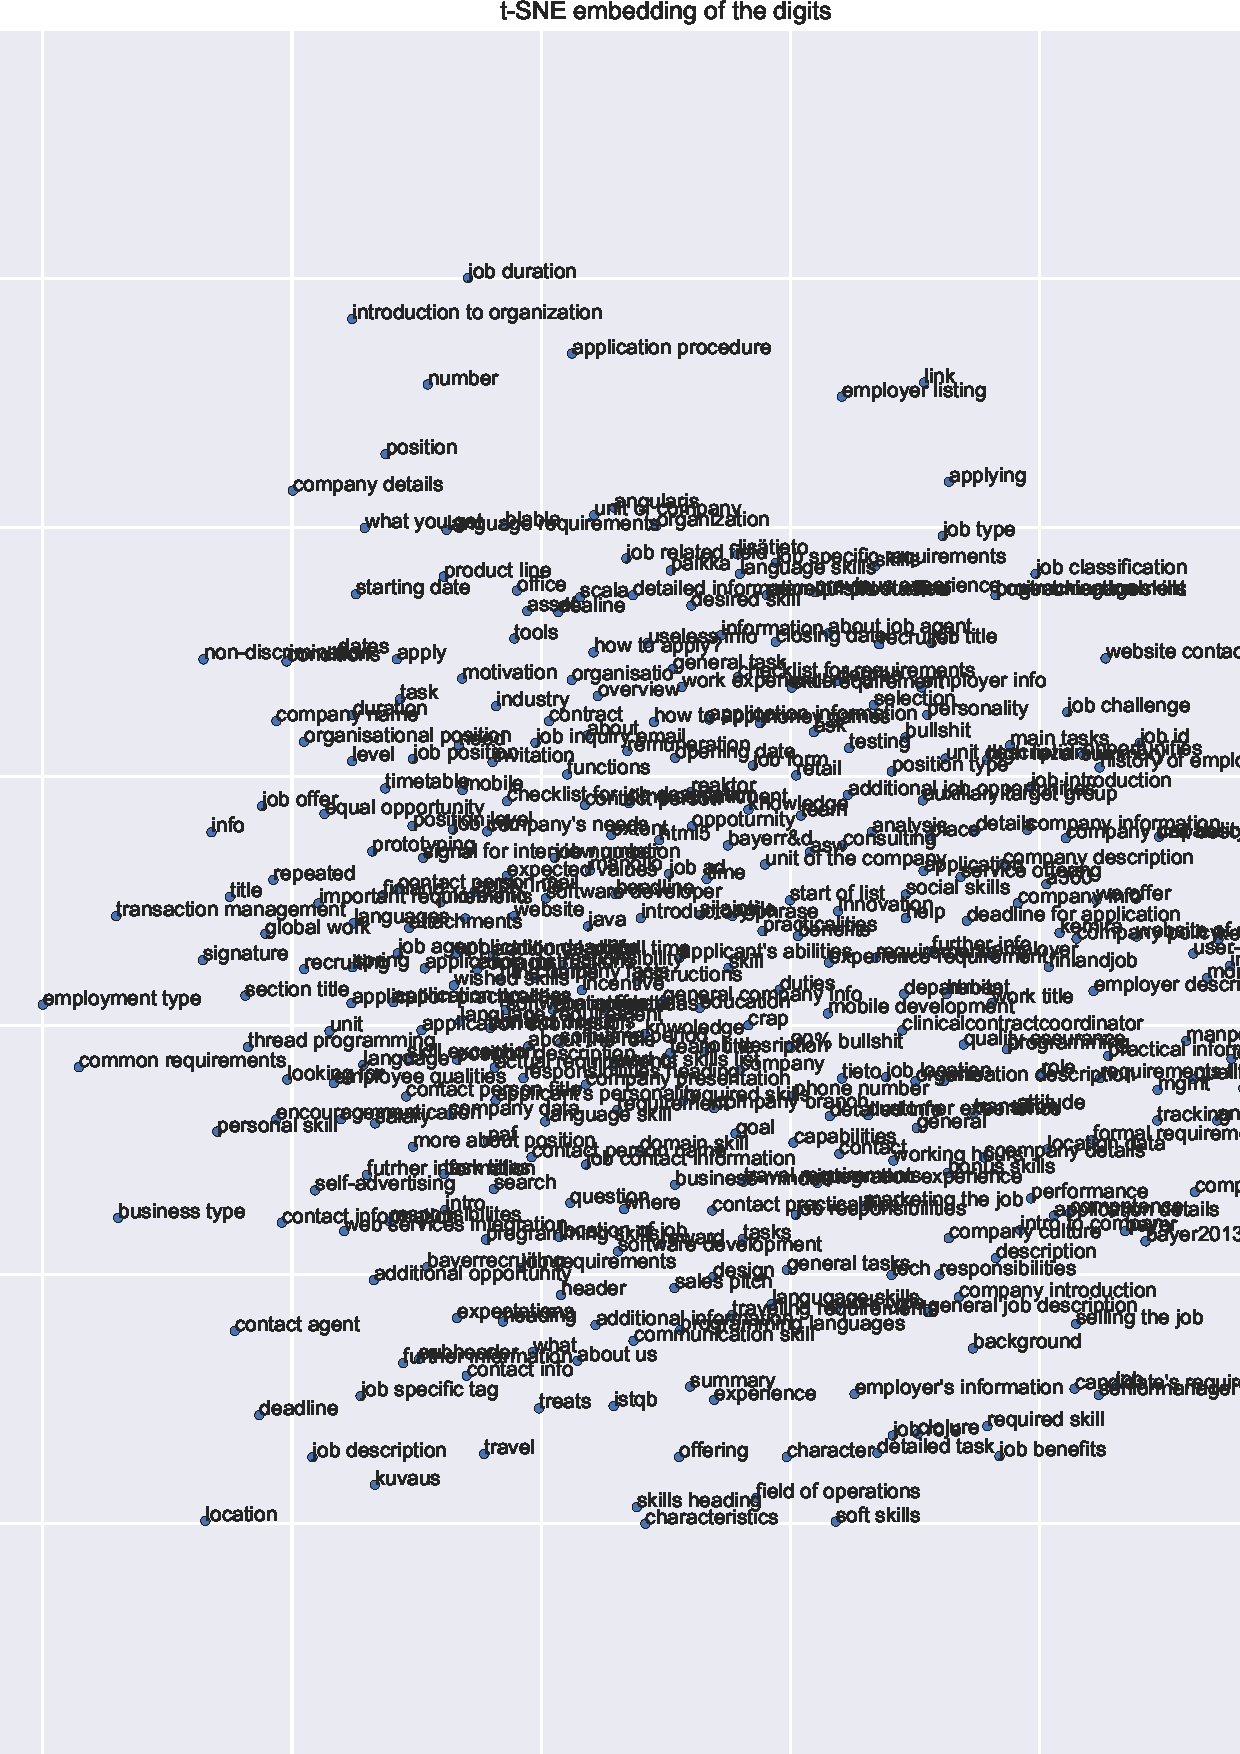
\includegraphics[width=\textwidth]{img/paragraph-data-tSNE.pdf}
    \caption{t-SNE Embedding}
\label{fig:paragraph-data-tSNE}
\end{figure}

\begin{figure}[h]
    \centering
    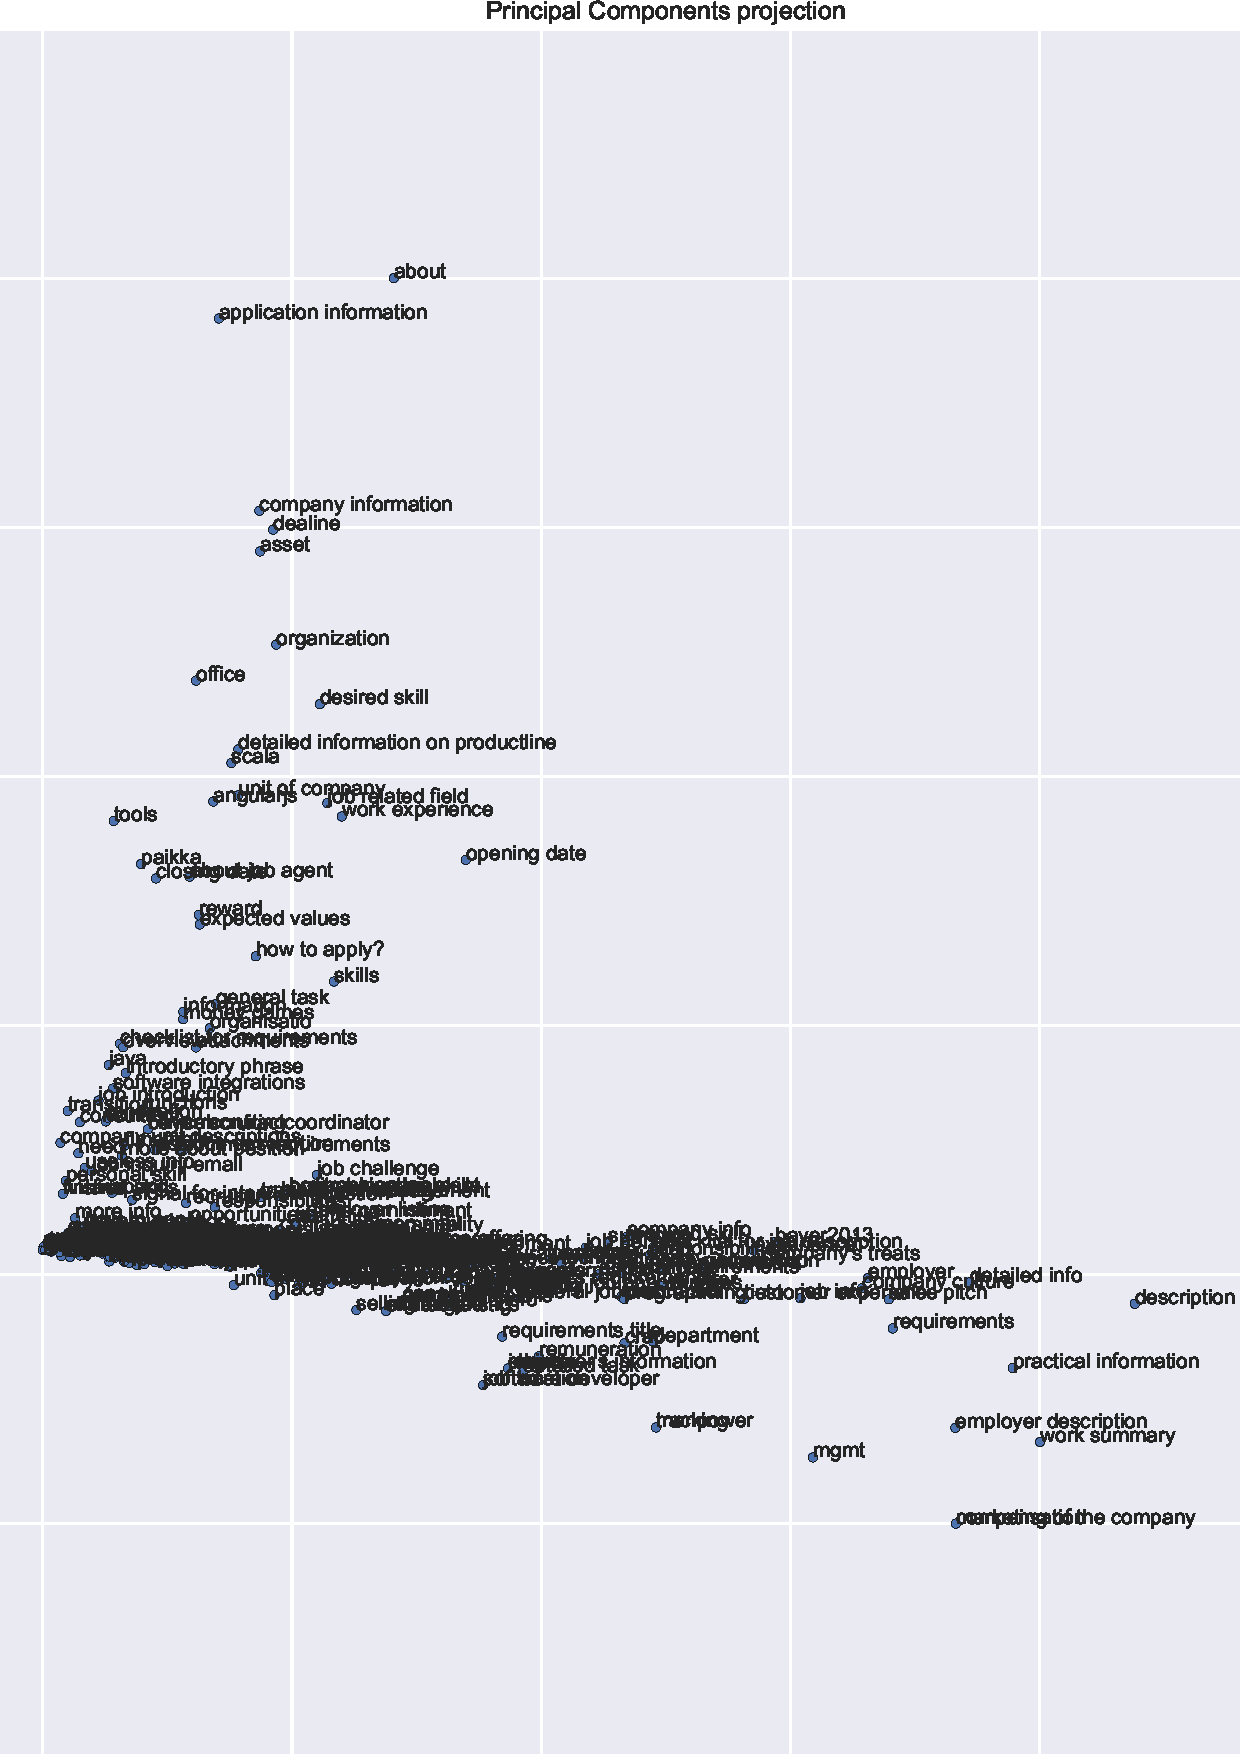
\includegraphics[width=\textwidth]{img/paragraph-data-principal-components-projection.pdf}
    \caption{Principal Components Projection}
\label{fig:paragraph-data-principal-components-projection}
\end{figure}

\todo{Comparison one-vs-rest and one-vs-one against linear machine}
\todo{Visualizations and embeddings of data in 2D (and decision boundaries?)}
\todo{show T-SNE embeddings of doc2vec vectors}

% !TEX root = ../thesis.tex
% !TEX spellcheck = en-US

\clearpage

\section{Explorative Experiments with Paragraph Dataset}

\section{Experiments with Sentence Dataset}

\subsection{Vector Space Models compared}


\todo{say why using the sentence dataset here}
\todo{reference jupyter notebook here}
% http://localhost:8888/notebooks/thesis/experiments/vector-space-models/Vector%20Space%20Models.ipynb#Setup

As Section~\ref{sec:vector-space-models} explains, a popular way to approach text classification and other tasks in natural language processing is to build a language model by creating explicit representations of the objects or entities to be processed in a vector space. Such vectors can be used as features for a learning algorithm. Depending on the representation they can also carry further meaning, such as to encode notions of similarity of associativity between the objects.

In order to determine effective vector space representations for the task of sentence classification, a set of experiments was carried out to study and compare different approaches. Each method was studied with regards to the effect of its hyper-parameters on effectiveness when producing an input space to different classifiers, but also time and memory requirements at training and inference time are taken into account \todo{actually discuss time and memory requirements}.

In order to compare the effectiveness for the sentence classification task as discussed in ?\todo{reference section here} each labelled document was transformed into a vector space representation using the different methods and then used for classification with a simple logistic regression classifier (\todo{link to logistic regression classifier explanation here}). Performance was then compared with regards to Matthews Correlation Coefficient for K classes (Section~\ref{par:Matthews Correlation Coefficient for K classes}) and the Accuracy \todo{link accuracy?} of the classifier.

\subsubsection{Baselines Classifiers: Uniform and Stratified Guessing}
\label{subs:baselines-classifiers}

As a baseline for comparing the performance of classification two different guessing strategies were used, namely uniform and stratified guessing.
Uniform guessing refers to a predictor that samples from the given classes assuming a uniform distribution whereas stratified guessing takes the label distribution in the data as the underlying probability distribution.
Then both methods just sample from these distributions to produce ``predictions'', while ignoring the actual input data. Both, uniform and stratified guessing achieve a Matthews Correlation Coefficient score of around 0 (averaged over 1000 runs) as expected for guessing strategies (see Section~\ref{subs:informedness-markedness-mcc}). On the other hand the accuracy for uniform guessing is around 0.16 which corresponds to $1/\text{K}$ for the K classes and around 0.26 for stratified guessing which reflects the skew of the label distribution.
Figure~\ref{fig:exp-vector-space-conf-matrix-guessing} shows the confusion matrices for these baseline variants in absolute and normalized form, revealing the properties of these guessing strategies.

\begin{figure}[h]
 % From http://localhost:8888/notebooks/thesis/experiments/vector-space-models/Vector%20Space%20Models.ipynb#Baseline:-Guessing-Strategies
    \centering
    \begin{subfigure}[b]{0.47\textwidth}
        \includegraphics[width=\textwidth]{img/exp-vector-space-conf-matrix-guessing-uniform.pdf}
        \caption{Uniform, absolute}
    \label{fig:exp-vector-space-conf-matrix-guessing-uniform}
    \end{subfigure}
~
    %add desired spacing between images, e. g. ~, \quad, \qquad, \hfill etc.
    %(or a blank line to force the subfigure onto a new line)
    \begin{subfigure}[b]{0.48\textwidth}
        \includegraphics[width=\textwidth]{img/exp-vector-space-conf-matrix-guessing-uniform-normalized.pdf}
        \caption{Uniform, normalized}
      \label{fig:exp-vector-space-conf-matrix-guessing-uniform-normalized}
    \end{subfigure}
~
    \begin{subfigure}[b]{0.47\textwidth}
        \includegraphics[width=\textwidth]{img/exp-vector-space-conf-matrix-guessing-stratified.pdf}
        \caption{Stratified, absolute}
      \label{fig:exp-vector-space-conf-matrix-guessing-stratified}
    \end{subfigure}
~
    %add desired spacing between images, e. g. ~, \quad, \qquad, \hfill etc.
    %(or a blank line to force the subfigure onto a new line)
    \begin{subfigure}[b]{0.48\textwidth}
        \includegraphics[width=\textwidth]{img/exp-vector-space-conf-matrix-guessing-stratified-normalized.pdf}
        \caption{Stratified, normalized}
      \label{fig:exp-vector-space-conf-matrix-guessing-stratified-normalized}
    \end{subfigure}
    \caption{Confusion matrices of uniform and stratified guessing strategies. }
\label{fig:exp-vector-space-conf-matrix-guessing}
\end{figure}

\subsubsection{N-gram Language Models}

The first class of language models that was investigated for the task of multi-class classification are N-gram models that were explained in Section~\ref{subs:n-gram-language-models}. As mentioned, in essence this type of model relies on simple statistics which makes for straightforward computation but at the same time comes at cost of expressiveness, especially in terms of temporal dependencies between words.

As N-grams models come in a variety of variants the most important ones were used as hyper-parameters to the model and a grid search was carried out over a wide range of combinations over these. The specific hyper-parameter settings are listed in Table~\ref{tab:ngram-parameters}. The grid search was optimized with regards to \emph{Matthews Correlation Coefficient} (see Section~\ref{par:Matthews Correlation Coefficient for K classes}) using 5-fold cross-validated with three standard classifiers: Logistic Regression and Naive Bayes and SVM.

\begin{table}[h]
  \begin{center}
  \begin{tabular}{ l l l}
    \toprule
    Hyper-Parameter & N-gram Type: Words & N-gram Type: Characters \\
    \midrule
    N-gram Range (Range) & [1,1], [1,2], [1,3], [2,3], [3,3] & [1,5], [1,10], [5,10], [5,15] \\
    Stop Words & English, None & N/A \\
    Vector Size (Size) & 10, 100, 300 & 10, 100, 300 \\
    IDF & Yes, No & Yes, No \\
    Norm & L1, L2, None & L1, L2, None \\
    Sub-linear TF & Yes, No & Yes, No \\
    \bottomrule
  \end{tabular}
  \caption{Parameter search space word and character level N-gram models}
  \label{tab:Ngram Parameters}
\end{center}
\end{table}

The 5 best results of these exhaustive grid searches can be seen in Table~\ref{tab:Ngram Grid Search} below.

\begin{table}[h]
  \begin{center}
  \begin{tabular}{ l l l l l l l l }
    \toprule
    Type & Range & Stop words & Size & IDF & Norm & Sub-linear TF & MCC Score \\
    \midrule
    Word & [1,1] & None & 300 & Yes &  & Yes & 0.689 \\
    Word & [1,1] & None & 300 & Yes &  & No & 0.687 \\
    Word & [1,1] & None & 300 & No &  & Yes & 0.682 \\
    Word & [1,1] & None & 300 & No &  & No & 0.682 \\
    Word & [1,1] & None & 300 & Yes & L2 & Yes & 0.68 \\
    % Word & [1,1] & None & 300 & Yes & L2 & No & 0.678 \\
    % Word & [1,2] & None & 300 & No &  & Yes & 0.677 \\
    % Word & [1,2] & None & 300 & Yes & L2 & Yes & 0.676 \\
    % Word & [1,2] & None & 300 & Yes & L2 & No & 0.675 \\
    % Word & [1,2] & None & 300 & No &  & No & 0.675 \\
    \midrule
    Word & [1,1] & None & 300 & No & & Yes & 0.659  \\
    Word & [1,1] & None & 300 & No & & No & 0.656 \\
    Word & [1,2] & None & 300 & No & & Yes & 0.655 \\
    Word & [1,2] & None & 300 & No & & No & 0.655 \\
    Word & [1,3] & None & 300 & No & & No & 0.65 \\
    % Word & [1,1] & None & 300 & Yes & L2 & Yes & 0.648 \\
    % Word & [1,1] & None & 300 & Yes & L2 & No & 0.648 \\
    % Word & [1,3] & None & 300 & No & & Yes & 0.648 \\
    % Word & [1,2] & None & 300 & Yes & L2 & No & 0.647 \\
    % Word & [1,2] & None & 300 & Yes & L2 & Yes & 0.646 \\
    \midrule
    Word & [1,1] & None & 300 & Yes & & Yes & 0.689 \\
    Word & [1,1] & None & 300 & Yes & & No  & 0.689 \\
    Word & [1,2] & None & 300 & Yes & & Yes & 0.677 \\
    Word & [1,2] & None & 300 & Yes & & No  & 0.677 \\
    Word & [1,3] & None & 300 & Yes & & Yes & 0.674 \\
    % Word & [1,3] & None    & 300 & Yes & & No  & 0.673 \\
    % Word & [1,1] & English & 300 & Yes & & Yes & 0.65 \\
    % Word & [1,1] & English & 300 & Yes & & No  & 0.65 \\
    % Word & [1,2] & English & 300 & Yes & & No  & 0.649 \\
    % Word & [1,2] & English & 300 & Yes & & Yes & 0.648 \\
    \bottomrule
  \end{tabular}
  \caption{Top 5 results of grid search over hyper-parameter space as listed in Table~\ref{tab:Ngram Parameters} using 5-fold cross-validated Logistic Regression (top), Naive Bayes (middle) and SVM (bottom) classifiers.}
\label{tab:Ngram Grid Search}
\end{center}
\end{table}

\todo{Why are the grid scores lower than the latter scores on the train/test split? Because they're averaged and only on the training data?}

Across all classifiers the following results on the hyper-parameters can be observed:

\paragraph{Type}
\label{par:Type}
Words as the atomic unit for N-grams consistently lead to better results. This is understandable as the search space of combinations of characters is significantly larger than the search space of known words.

\paragraph{Range}
\label{par:Range}
There are slight differences to be observed between the three classifiers used, but with all three models the best performance is achieved using Unigrams. Also all of the top results across all classifiers include Unigrams in the model while extending the range towards bigrams or trigrams.

\paragraph{Stop Words}
\label{par:Stop Words}
None of the top results of the performed grid searches used stop words. This is interesting as using stop-words to remove hand-picked, highly frequent words that do not carry much meaning is common practice. It seems there is information carried within these stop words. Of course this outcome is also influenced by the particular stop-list used (see Section~\ref{subp:Stop words}).

\paragraph{Size (matters)}
\label{par:Size}
For the searched settings the largest vector dimensionality of 300 achieves the best performance. This is not surprising as higher-dimensional vectors can capture more information about N-gram occurrences. However in practice the vector size must be limited as it grows with the vocabulary -- potentially at an exponential rate if N-grams other than Unigrams are used. Also very high dimensionality often leads to decreased performance in terms of generalization of the model.

\paragraph{IDF}
\label{par:IDF}
There is no consensus between the classifiers on whether or not to weigh the N-gram frequencies by the \emph{inverse document frequency} (see Section~\ref{subp:TF.IDF weighting}). Thus it seems advisable to lead this parameter free for and evaluate both variants with a given classifier. For logistic regression however the performance differences are marginal and so the choice for this parameter seems somewhat arbitrary.

\paragraph{Norm}
\label{par:Norm}
Is seems that normalizing the vectors in most cases does not lead to any performance gains. Again this is an often recommended practice but here it does not seem to add any value to the model.

\paragraph{Sub-linear TF}
\label{par:Sub-linear TF}
Applying sub-linear TF (see Section~\ref{subp:Sublinear TF scaling}) does not seem to affect the results much and the choice of this parameter can hence be chosen almost arbitrarily as well, although here for all three classifiers applying it leads to a marginal improvement.

Table~\ref{tab:Ngram Grid Search Scores} shows the scores of each classifier using the best N-gram model. It is evident that here logistic regression actually performs best as it offers both, a good accuracy as well as the highest score for Matthews Correlation Coefficient.

\begin{table}[h]
  \begin{center}
  \begin{tabular}{ r | *2l | *2l }
    \toprule
     & \multicolumn{2}{c|}{Training} & \multicolumn{2}{|c}{Validation}\\
    Classifier & Accuracy & MCC & Accuracy & MCC \\
    \midrule
    Logistic Regression & 0.824 & 0.761 & 0.787 & 0.708 \\
    Naive Bayes         & 0.769 & 0.681 & 0.767 & 0.677 \\
    SVM                 & 0.835 & 0.681 & 0.786 & 0.700 \\
    \bottomrule
  \end{tabular}
  \caption{Performance of each best N-gram model with Logistic Regression and Naive Bayes on the validation data}
\label{tab:Ngram Grid Search Scores}
\end{center}
\end{table}

\begin{figure}[h]
    \centering
    \begin{subfigure}[b]{0.32\textwidth}
        \includegraphics[width=\textwidth]{img/exp-vector-space-conf-matrix-ngram-logreg-normalized.pdf}
        \caption{Logistic Regression}
        \label{fig:exp-vector-space-conf-matrix-ngram-logreg-normalized}
    \end{subfigure}
    \begin{subfigure}[b]{0.32\textwidth}
        \includegraphics[width=\textwidth]{img/exp-vector-space-conf-matrix-ngram-naivebayes-normalized.pdf}
        \caption{Naive Bayes}
        \label{fig:exp-vector-space-conf-matrix-ngram-naivebayes-normalized}
    \end{subfigure}
    \begin{subfigure}[b]{0.32\textwidth}
        \includegraphics[width=\textwidth]{img/exp-vector-space-conf-matrix-ngram-svm-normalized.pdf}
        \caption{SVM}
        \label{fig:exp-vector-space-conf-matrix-ngram-svm-normalized}
    \end{subfigure}
    \caption{Normalized confusion matrices all three classifiers using the best N-gram model found via cross-validated grid search. Both Naive Bayes as well as SVM show label bias towards the prevalent class \emph{candidate}.}
  \label{fig:exp-vector-space-conf-matrix-ngram}
\end{figure}
\todo{properly align visualization}

Figure~\ref{fig:exp-vector-space-ngram} shows projections of the of the constructed feature space using the best model that was optimized with Logistic Regression. This visualization shows the separability of the classes in this space. Especially the PCA projection here reveals that it is clearly possible to separate the classes until a certain point.

\begin{figure}[h]
    \centering
    \begin{subfigure}[b]{0.48\textwidth}
      \includegraphics[width=\textwidth]{img/exp-vector-space-ngram-pca.pdf}
      \caption{PCA projection}
      \label{fig:exp-vector-space-ngram-pca}
    \end{subfigure}
    ~
    %add desired spacing between images, e. g. ~, \quad, \qquad, \hfill etc.
    %(or a blank line to force the subfigure onto a new line)
    \begin{subfigure}[b]{0.48\textwidth}
      \includegraphics[width=\textwidth]{img/exp-vector-space-ngram-tsne.pdf}
      \caption{t-SNE projection}
      \label{fig:exp-vector-space-ngram-tsne}
    \end{subfigure}
    \caption{Document vectors produced by the best N-gram model (optimized w.r.t. Logistic Regression) projected onto the first 2 principal components (left) and project using t-SNE projection.}
  \label{fig:exp-vector-space-ngram}
\end{figure}

\subsubsection{Bag-of-Means - An Averaged Word2Vec Model}

Next a Bag-of-Means model as described in Section~\ref{subp:Bag-of-Means} was evaluated with the same set of classifiers. The model was evaluated on the same test and training data split as used for the N-gram model above. As a basis the pre-trained word-vectors from the Google News dataset\footnote{The dataset contains contains 300-dimensional vectors for 3 million words and phrases. The phrases were obtained using a simple data-driven approach described in~\cite{Mikolov:2013ab}. The dataset can be obtained on the following website: \url{https://code.google.com/archive/p/word2vec/}} were used and then for each document all word vectors were average to obtain the document vector. The results can be seen in Table~\ref{tab:Bag-Of-Means Results}.

\begin{table}[h]
  \begin{center}
  \begin{tabular}{ r | *2l | *2l }
    \toprule
     & \multicolumn{2}{c|}{Training} & \multicolumn{2}{|c}{Validation}\\
    Classifier & Accuracy & MCC & Accuracy & MCC \\
    \midrule
    Logistic Regression & 0.797 & 0.722 & 0.784 & 0.702 \\
    Naive Bayes         & 0.337 & 0.271 & 0.320 & 0.251 \\
    SVM                 & 0.545 & 0.356 & 0.562 & 0.379 \\
    \bottomrule
  \end{tabular}
  \caption{Performance base classifiers using the Bag-of-Means model}
\label{tab:Bag-Of-Means Results}
\end{center}
\end{table}

The model performs well using Logistic Regression and is almost on par with the best N-gram model. This is surprising as performance previously reported to be rather poor as mention in Section~\ref{subp:Bag-of-Means}. On the other hand the variance in results between the classifiers is huge and especially Naive Bayes seems to perform extremely poor. Further investigation into the use of different classifiers could shed light into these diverging results which are not observed using the N-gram models in the section above. The confusion matrices in Figure~\ref{fig:exp-vector-space-conf-matrix-bom} reveal strong label bias in the case of Naive Bayes and SVM, although it is unclear where this stems from. Figure~\ref{fig:exp-vector-space-bom} makes clear though that there is a somewhat meaningful mapping into the feature space. \todo{mention one-vs-all scheme for log reg? also for ngrams above}

\begin{figure}[h]
    \centering
    \begin{subfigure}[b]{0.32\textwidth}
        \includegraphics[width=\textwidth]{img/exp-vector-space-conf-matrix-bom-logreg-normalized.pdf}
        \caption{Logistic Regression}
        \label{fig:exp-vector-space-conf-matrix-bom-logreg-normalized}
    \end{subfigure}
    \begin{subfigure}[b]{0.32\textwidth}
        \includegraphics[width=\textwidth]{img/exp-vector-space-conf-matrix-bom-naivebayes-normalized.pdf}
        \caption{Naive Bayes}
        \label{fig:exp-vector-space-conf-matrix-bom-naivebayes-normalized}
    \end{subfigure}
    \begin{subfigure}[b]{0.32\textwidth}
        \includegraphics[width=\textwidth]{img/exp-vector-space-conf-matrix-bom-svm-normalized.pdf}
        \caption{SVM}
        \label{fig:exp-vector-space-conf-matrix-bom-svm-normalized}
    \end{subfigure}
    \caption{Normalized confusion matrices of all three classifiers using the Bag-of-Means model.}
  \label{fig:exp-vector-space-conf-matrix-bom}
\end{figure}

\begin{figure}[h]
    \centering
    \begin{subfigure}[b]{0.48\textwidth}
      \includegraphics[width=\textwidth]{img/exp-vector-space-bom-pca.pdf}
      \caption{PCA projection}
      \label{fig:exp-vector-space-bom-pca}
    \end{subfigure}
    ~
    %add desired spacing between images, e. g. ~, \quad, \qquad, \hfill etc.
    %(or a blank line to force the subfigure onto a new line)
    \begin{subfigure}[b]{0.48\textwidth}
      \includegraphics[width=\textwidth]{img/exp-vector-space-bom-tsne.pdf}
      \caption{t-SNE projection}
      \label{fig:exp-vector-space-bom-tsne}
    \end{subfigure}
    \caption{Document vectors produced by Bag-of-Means model (optimized w.r.t. Logistic Regression) projected onto the first 2 principal components (left) and projected using t-SNE projection. It is clear that even though the vectors are simply obtained by averaging they do indeed produce somewhat seperable manifolds.}
  \label{fig:exp-vector-space-bom}
\end{figure}

\subsubsection{Paragraph Vectors using Distributed Representations}

Next a vector space model was build using the approach proposed by  \cite{Le:2014aa} and described in more detail in Section~\ref{par:Distributed representations for documents}. Again there are several hyper-parameters to this model that are described in Section~\ref{subs:Language Models using Distributed Representations} and turn out to have a huge influence on its performance as the results below indicate. As this model is computationally quite expensive a grid search as for the N-gram model above was infeasible. Thus the effect of the hyper-parameters was studied by just varying them one at a time while keeping the others fixed, using a Logistic Regression classifier with 5-fold cross-validation. The next sections will briefly outline the results of these tests:

\paragraph{Vector Size}
As was to expect the vector size of the model correlates with the performance. Again the highest chosen dimensionality was 300 which yielded the best results with a Matthews Correlation Coefficient of 0.53, however the difference to a 100-dimensional model was marginal with 1\% absolute improvement. Surprisingly even a 10-dimensional vector space model is capable of achieving almost best results with a difference of only 2\% to the 300-dimensional model. Even a 2-dimensional model could achieve a MCC score of 14\%.

\begin{table}[h]
  \begin{center}
  \begin{tabular}{ *6l | l }
    \toprule
    type & size & window & negative & hs & sample & MCC  \\
    \midrule
    PV-DM & 2 & 2   & 3 & 1 & 0 & 0.536 \\
    PV-DM & 2 & 10  & 3 & 1 & 0 & 0.522 \\
    PV-DM & 2 & 100 & 3 & 1 & 0 & 0.514 \\
    PV-DM & 2 & 300 & 3 & 1 & 0 & 0.144 \\
    \bottomrule
  \end{tabular}
  \caption{Matthews Correlation Coefficient with varying vector size. The abbreviations are as follows: Model Type, i.e. PV-DM vs. PV-DBOW (type),  Vector Size (size), Window Size (size), Negative Sampling value $k$ (negative), Hierarchical Softmax used (hs), Frequent word sub-sampling threshold (sample).}
\label{tab:Paragraph Vector Parameter Results Size}
\end{center}
\end{table}

\paragraph{Frequent Word Sub-Sampling}
Frequent word sub-sampling can boost performance quite much, but again choosing the right value for this hyper-parameter is key. The training behavior with different sampling thresholds differs quite much. Figure~\ref{fig:exp-vector-space-doc2vec-param-sample} shows the training with different values with 100 passes over the dataset. A good value seems to be $10^{-5}$ which achieves an MCC score of 0.697 and is on-par with the best N-gram model. Interestingly not using sub-sampling in this setup seemed to be overfitting as the score decreases quite drastically with more training passes. A similar effect is observed with a higher threshold of $10^{-4}$ but much less strong. Choosing a lower threshold of $10^{-6}$ leads to very poor performance with an MCC score of only 0.07.

\begin{table}[h]
  \begin{center}
  \begin{tabular}{ *6l | l }
    \toprule
    type & size & window & negative & hs & sample & MCC  \\
    \midrule
    PV-DM & 300 & 10 & 3 & 1 & 0 & 0.244 \\
    PV-DM & 300 & 10 & 3 & 1 & 1e-4 & 0.556 \\
    PV-DM & 300 & 10 & 3 & 1 & 1e-5 & 0.698 \\
    PV-DM & 300 & 10 & 3 & 1 & 1e-6 & 0.071 \\
    \bottomrule
  \end{tabular}
  \caption{Matthews Correlation Coefficient with varying frequent word sub-sampling threshold. The abbreviations are as follows: Model Type, i.e. PV-DM vs. PV-DBOW (type),  Vector Size (size), Window Size (size), Negative Sampling value $k$ (negative), Hierarchical Softmax used (hs), Frequent word sub-sampling threshold (sample).}
\label{tab:Paragraph Vector Parameter Results Sample}
\end{center}
\end{table}

\begin{figure}[h]
    \centering
    \includegraphics[width=\textwidth]{img/exp-vector-space-doc2vec-param-sample.pdf}
    \caption{Training of document vectors with different sub-sampling thresholds.}
  \label{fig:exp-vector-space-doc2vec-param-sample}
\end{figure}

\paragraph{Hierarchical Softmax}
Using hierarchical softmax increased the performance, leading to a 12\% absolute difference in terms of MCC score.

\begin{table}[h]
  \begin{center}
  \begin{tabular}{ *6l | l }
    \toprule
    type & size & window & negative & hs & sample & MCC  \\
    \midrule
    PV-DM & 100 & 10 & 3 & 0 & 0 & 0.398 \\
    PV-DM & 100 & 10 & 3 & 1 & 0 & 0.520 \\
    \bottomrule
  \end{tabular}
  \caption{Matthews Correlation Coefficient with and without using hierarchical softmax. The abbreviations are as follows: Model Type, i.e. PV-DM vs. PV-DBOW (type),  Vector Size (size), Window Size (size), Negative Sampling value $k$ (negative), Hierarchical Softmax used (hs), Frequent word sub-sampling threshold (sample).}
\label{tab:Paragraph Vector Parameter Results Hierarchical Softmax}
\end{center}
\end{table}

\paragraph{Negative Sampling}
Negative Sampling generally increased the performance of the model and smaller values actually worked best out of the tested settings from 0 to 6. Choosing the number of negative samples to be 2 resulted in the best performance, but the absolute difference in performance was only about 6\% of achieved MMC score.

\begin{table}[h]
  \begin{center}
  \begin{tabular}{ *6l | l }
    \toprule
    type & size & window & negative & hs & sample & MCC  \\
    \midrule
    PV-DM & 100 & 10 & 0 & 1 & 0 & 0.530 \\
    PV-DM & 100 & 10 & 1 & 1 & 0 & 0.541 \\
    PV-DM & 100 & 10 & 2 & 1 & 0 & 0.536 \\
    PV-DM & 100 & 10 & 3 & 1 & 0 & 0.524 \\
    PV-DM & 100 & 10 & 4 & 1 & 0 & 0.516 \\
    PV-DM & 100 & 10 & 5 & 1 & 0 & 0.498 \\
    PV-DM & 100 & 10 & 6 & 1 & 0 & 0.482 \\
    \bottomrule
  \end{tabular}
  \caption{Matthews Correlation Coefficient with varying negative sampling value. The abbreviations are as follows: Model Type, i.e. PV-DM vs. PV-DBOW (type),  Vector Size (size), Window Size (size), Negative Sampling value $k$ (negative), Hierarchical Softmax used (hs), Frequent word sub-sampling threshold (sample).}
\label{tab:Paragraph Vector Parameter Results Hierarchical Softmax}
\end{center}
\end{table}

\paragraph{Window Size}
Window sizes of 5, 10 and 15 were experimented with which increase or decrease the width of context the model is trained on. Here a window size of 10 showed best results. It is safe to assume that increasing the window size much further does not lead to any improvement in the model as the correlation with the word should become weaker the farther we move away from it in a document or text.


\begin{table}[h]
  \begin{center}
  \begin{tabular}{ *6l | l }
    \toprule
    type & size & window & negative & hs & sample & MCC  \\
    \midrule
    PV-DM & 100 & 5 & 3 & 1 & 0 & 0.508 \\
    PV-DM & 100 & 10 & 3 & 1 & 0 & 0.523 \\
    PV-DM & 100 & 15 & 3 & 1 & 0 & 0.510 \\
    \bottomrule
  \end{tabular}
  \caption{Matthews Correlation Coefficient with varying window size. The abbreviations are as follows: Model Type, i.e. PV-DM vs. PV-DBOW (type),  Vector Size (size), Window Size (size), Negative Sampling value $k$ (negative), Hierarchical Softmax used (hs), Frequent word sub-sampling threshold (sample).}
\label{tab:Paragraph Vector Parameter Results Hierarchical Softmax}
\end{center}
\end{table}

\paragraph{PV-DBOW versus PM-DV}
Both models for paragraph vectors proposed in \cite{Le:2014aa} were tried, namely Distributed Bag of Words version of Paragraph Vector (PV-DBOW) and Distributed Memory version of Paragraph Vec- tor (PV-DM). In these tests the DBOW model achieves significantly better results with an MCC that is 14\% than the PV-DM model in absolute terms. This is in contrast with the results in the aforementioned paper, where the authors state that \textquote{PV-DM is consistently better than PV-DBOW.}~\cite{Le:2014aa}.

\begin{table}[h]
  \begin{center}
  \begin{tabular}{ *6l | l }
    \toprule
    type & size & window & negative & hs & sample & MCC  \\
    \midrule
    PV-DM & 100 & 10 & 3 & 1 & 0 & 0.521 \\
    PV-BBOW & 100 & 10 & 3 & 1 & 0 & 0.667 \\
    \bottomrule
  \end{tabular}
  \caption{Matthews Correlation Coefficient with varying window size. The abbreviations are as follows: Model Type, i.e. PV-DM vs. PV-DBOW (type),  Vector Size (size), Window Size (size), Negative Sampling value $k$ (negative), Hierarchical Softmax used (hs), Frequent word sub-sampling threshold (sample).}
\label{tab:Paragraph Vector Parameter Results Hierarchical Softmax}
\end{center}
\end{table}

\paragraph{Evaluating the best hyper-parameter setting}

\subsubsection{Paragraph Vectors using pre-initialized weights *}

\subsubsection{Paragraph Vectors using context sentences *}

\subsubsection{Results and Discussion *}




\subsection{Finding the best Classifier using Vector Space Models}

\subsection{Advanced and experimental approaches}

\subsubsection{Inversion of Distributed Language Representations}

\subsubsection{LSTM Multi-task learner}
\label{subs:LSTM Multi-task learner}

% !TEX root = ../thesis.tex
% !TEX spellcheck = en-US

\clearpage
\section{Discussion and Conclusions}

\subsection{Discussion of Experimental Results}

\subsection{Conclusions}
\label{subs:conclusions}

\begin{itemize}
  \item As in many areas of machine learning much work has been going into feature engineering but it seems that feature learning, while much more computationally expensive, surpasses the potential of engineered feature representations. Deep learning and meta-learning are mature enough to make up for the gap that has been there for years: To achieve performance that is good enough to make an algorithmic system usable in production, huge amounts of research and engineering went into feature engineering and finally the performance of these methods can be matched and even surpassed by automated methods or learning features. (link here NG's transfer learning work, also Schmidhubers work of meta-learning and on function prediction etc)
  \item There is more need to understand the representations of such feature learning systems though, statistics are quite easy to understand but weights of a neural network don't tell much. There is however potential for learning ``better statistics'' ourselves, e.g. how to efficiently learn a language (by looking at explicit indermediate representations of the states of a NN)
  \item
\end{itemize}


\subsection{Contributions}
\label{sub:contributions}

\begin{itemize}
  \item compare n-gram and doc2vec (?)
  \item
\end{itemize}

\subsection{Proposal for Future Research}
\label{sub:further-research}

\begin{itemize}
  \item how well do word2vec and comparable methods generalize: e.g.\ initialize a text corpus with word vectors from a bigger corpus (Google News), then train an RNN to predict the next word vector using the small corpus but use the bigger corpus to validate and see if words in bigger corpus can be inferred
  \item trajectory based algorithms (word trajectory through space for a sentence)
  \item Compare with standard benchmarks (TREC etc)
  \item Meta- / Transfer-learning: OCR with simultaneous LM learning (e.g. predict next character)
\end{itemize}

\paragraph{Trajectory -Based Algorithms on Text}
\label{par:Trajectory Algorithms on Text}
As shown in \cite{Mikolov:2013ac} and related work that was outlined in Section\todo{reference here} vector space models for text can capture very subtle semantic relationships between words by their location in the vector space. When


\subsection{Learnings}
\label{sub:learnings}

\begin{itemize}
  \item focusing on both, building a working system (engineering) and exploring new directions (science), is hard
  \item problem framing is hard
\end{itemize}


%% Bibliography

\clearpage
%% The \phantomsection command is nessesary for hyperref to jump to the
%% correct page, in other words it puts a hyper marker on the page.
\phantomsection
\addcontentsline{toc}{section}{\refname}
%\addcontentsline{toc}{section}{References}
\bibliography{literature/thesis-research.bib}
\bibliographystyle{apalike}
%\nocite{*}

%% Appendix

\include{./tex/7_appendix.tex}

\end{document}
